\section{Experiments}
\label{sec:experiments}

The experiments answer three questions.
\textbf{RQ1}: does critique-guided rewriting improve on-policy distillation on
held-out mathematical reasoning benchmarks, and does it preserve performance
outside mathematics?
\textbf{RQ2}: which components of \ours{} account for the improvement?
\textbf{RQ3}: where do the gains of \ours{} come from?
Section~\ref{sec:experiments-setup} describes the shared setup, and the
following subsections answer each question in turn.


\subsection{Setup}
\label{sec:experiments-setup}

\noindent\textbf{Models and training.}
We distill Qwen3-1.7B and Qwen3-0.6B, both in non-thinking mode, from the
Qwen3-4B-Instruct-2507 teacher on the prompts of DAPO-Math-17k.
All methods within a student scale share the same training recipe.
\ours{} uses the teacher as the critic, and the critic lists all errors that it
finds in the solution of the student within a limit of $2{,}048$ tokens.
Appendix~\ref{app:setup} gives the hyperparameters, and
Appendix~\ref{app:prompts} lists the prompts.

\noindent\textbf{Baselines.}
We compare four classes of baselines.
The first class contains standard post-training methods.
SFT and KD train on solutions of the teacher, GRPO uses an outcome
reward without the teacher, and OPD performs standard on-policy distillation.

The second class uses privileged information during
training, as CriticOPD does. OPSD-T
\citep{zhao2026selfdistilled} lets the teacher score
student rollouts with the reference answer in its
context. Critique-GRPO \citep{zhang2026critiquegrpo}
lets the student revise incorrect solutions with
teacher critiques and optimizes the original and
revised solutions with outcome rewards.
% TODO: replace the citation keys of OPSD-T (arXiv 2602.04942 / 2601.18734)
% and Critique-GRPO (arXiv 2506.03106).
The third and fourth classes correspond to the two responses to the loss of
recoverability that Section~\ref{sec:intro} describes.
The third class reduces supervision, and FastOPD \citep{zhang2026fast}
represents it by truncating long rollouts.
The fourth class replaces the sequence, and TRD \citep{jiang2026trajectory},
SKD \citep{xu2025speculative}, and RelayOPD \citep{xu2026relay} let the teacher
rewrite the solution of the student or write into its trajectory.

\noindent\textbf{Evaluation.}
We evaluate on AIME 2024, AIME 2025, AMC 2023, MATH500, OlympiadBench, and
Minerva Math with a budget of $32{,}768$ tokens.
We report the mean accuracy over $32$ samples per problem on the first three
benchmarks and over $8$ samples on the others.
We train each method with three seeds and report the mean and the standard
deviation at the checkpoint that we select under seed $42$
(Appendix~\ref{app:setup}).


\subsection{RQ1: Does critique-guided rewriting improve OPD?}
\label{sec:experiments-results}

\begin{table*}[t]
\centering
\caption{
\textbf{Results on six mathematical reasoning benchmarks.}
Entries are means and standard deviations over three seeds, and the subscript after each method gives the selected step.
Bold marks the best student at each scale.
}
\label{tab:main}

\scriptsize
\setlength{\tabcolsep}{3pt}
\renewcommand{\arraystretch}{1.05}

\begin{tabularx}{\textwidth}{l*{7}{>{\centering\arraybackslash}X}}
\toprule
\textbf{Method}
& \textbf{AIME24}
& \textbf{AIME25}
& \textbf{AMC23}
& \textbf{MATH500}
& \textbf{OlympiadBench}
& \textbf{Minerva}
& \textbf{Avg}
\\
\midrule

Teacher
& 62.19 & 48.12 & 85.99 & 94.83 & 72.26 & 45.54
& 68.16 \\

\midrule
\multicolumn{8}{c}{\textit{Student: Qwen3-0.6B-Non-Thinking}} \\
\midrule

Student
& 2.08 & 1.35 & 18.98 & 45.52 & 16.94 & 13.69
& 16.43 \\

\arrayrulecolor{black!35}\specialrule{0.35pt}{1.2pt}{1.2pt}\arrayrulecolor{black}

SFT$_{@139}$
& 4.62$_{\pm 0.49}$ & 6.84$_{\pm 0.12}$ & 30.08$_{\pm 0.20}$ & 58.60$_{\pm 0.37}$ & 27.24$_{\pm 0.20}$ & 15.59$_{\pm 0.25}$
& 23.83$_{\pm 0.06}$ \\

KD$_{@139}$
& 4.51$_{\pm 0.63}$ & 6.15$_{\pm 0.73}$ & 28.75$_{\pm 0.80}$ & 57.88$_{\pm 0.69}$ & 26.62$_{\pm 0.52}$ & 15.09$_{\pm 0.88}$
& 23.17$_{\pm 0.49}$ \\

GRPO$_{@80}$
& 3.82$_{\pm 0.71}$ & 3.78$_{\pm 1.27}$ & 26.46$_{\pm 0.92}$ & 53.72$_{\pm 1.60}$ & 23.45$_{\pm 1.14}$ & 15.12$_{\pm 0.71}$
& 21.06$_{\pm 1.00}$ \\

Critique-GRPO$_{@40}$
& 1.42$_{\pm 0.43}$ & 0.97$_{\pm 0.53}$ & 16.59$_{\pm 0.61}$ & 41.02$_{\pm 1.07}$ & 13.93$_{\pm 0.45}$ & 11.47$_{\pm 0.15}$
& 14.23$_{\pm 0.49}$ \\

\arrayrulecolor{black!35}\specialrule{0.35pt}{1.2pt}{1.2pt}\arrayrulecolor{black}

OPD$_{@40}$
& 10.24$_{\pm 1.17}$ & 14.69$_{\pm 1.36}$ & 45.14$_{\pm 0.64}$ & 72.93$_{\pm 0.32}$ & 42.42$_{\pm 0.79}$ & 23.35$_{\pm 0.20}$
& 34.80$_{\pm 0.30}$ \\

OPSD-T$_{@80}$
& 13.37$_{\pm 0.93}$ & 15.00$_{\pm 0.28}$ & 47.48$_{\pm 0.25}$ & 75.52$_{\pm 0.43}$ & 44.10$_{\pm 0.26}$ & 24.26$_{\pm 0.44}$
& 36.62$_{\pm 0.15}$ \\

\arrayrulecolor{black!35}\specialrule{0.35pt}{1.2pt}{1.2pt}\arrayrulecolor{black}

FastOPD$_{@40}$
& 13.72$_{\pm 0.95}$ & 18.75$_{\pm 0.91}$ & 47.43$_{\pm 0.94}$ & 75.18$_{\pm 0.29}$ & 44.48$_{\pm 0.65}$ & 24.17$_{\pm 0.63}$
& 37.29$_{\pm 0.46}$ \\

TRD$_{@139}$
& 3.75$_{\pm 0.31}$ & 5.35$_{\pm 0.37}$ & 27.85$_{\pm 0.51}$ & 55.14$_{\pm 0.55}$ & 25.72$_{\pm 0.60}$ & 14.86$_{\pm 0.25}$
& 22.11$_{\pm 0.25}$ \\

SKD$_{@40}$
& 7.78$_{\pm 0.63}$ & 10.38$_{\pm 0.53}$ & 36.19$_{\pm 0.45}$ & 65.60$_{\pm 0.21}$ & 33.81$_{\pm 0.53}$ & 19.41$_{\pm 0.56}$
& 28.86$_{\pm 0.24}$ \\

RelayOPD$_{@60}$
& 13.90$_{\pm 0.58}$ & 17.64$_{\pm 0.57}$ & 48.96$_{\pm 1.11}$ & 76.49$_{\pm 0.31}$ & 46.01$_{\pm 0.25}$ & \textbf{25.60}$_{\pm 0.44}$
& 38.10$_{\pm 0.22}$ \\

\rowcolor{blue!8}
\textbf{\ours{}}$_{@40}$
& \textbf{14.81}$_{\pm 0.73}$ & \textbf{19.41}$_{\pm 0.47}$ & \textbf{50.44}$_{\pm 0.48}$ & \textbf{76.56}$_{\pm 0.35}$ & \textbf{46.81}$_{\pm 0.51}$ & 25.14$_{\pm 0.26}$
& \textbf{38.86}$_{\pm 0.15}$ \\

\rowcolor{blue!8}
\textcolor{green!50!black}{$\Delta$ vs OPD}
& \textcolor{green!50!black}{+4.57}
& \textcolor{green!50!black}{+4.72}
& \textcolor{green!50!black}{+5.30}
& \textcolor{green!50!black}{+3.63}
& \textcolor{green!50!black}{+4.39}
& \textcolor{green!50!black}{+1.79}
& \textcolor{green!50!black}{+4.06}
\\

\midrule
\multicolumn{8}{c}{\textit{Student: Qwen3-1.7B-Non-Thinking}} \\
\midrule

Student
& 11.98 & 9.17 & 41.00 & 73.22 & 39.80 & 29.23
& 34.07 \\

\arrayrulecolor{black!35}\specialrule{0.35pt}{1.2pt}{1.2pt}\arrayrulecolor{black}

SFT$_{@40}$
& 27.71$_{\pm 1.00}$ & 23.37$_{\pm 1.03}$ & 58.82$_{\pm 0.40}$ & 83.39$_{\pm 0.38}$ & 52.58$_{\pm 0.42}$ & 34.56$_{\pm 0.09}$
& 46.74$_{\pm 0.48}$ \\

KD$_{@139}$
& 20.59$_{\pm 0.43}$ & 17.85$_{\pm 2.29}$ & 52.18$_{\pm 0.63}$ & 79.22$_{\pm 0.22}$ & 48.50$_{\pm 0.46}$ & 33.79$_{\pm 0.92}$
& 42.02$_{\pm 0.49}$ \\

GRPO$_{@120}$
& 26.94$_{\pm 1.59}$ & 20.80$_{\pm 1.20}$ & 56.22$_{\pm 0.43}$ & 82.21$_{\pm 0.98}$ & 52.15$_{\pm 1.04}$ & 33.95$_{\pm 0.53}$
& 45.38$_{\pm 0.85}$ \\

Critique-GRPO$_{@40}$
& 9.83$_{\pm 0.57}$ & 8.58$_{\pm 0.39}$ & 38.24$_{\pm 0.28}$ & 70.11$_{\pm 0.34}$ & 35.90$_{\pm 0.25}$ & 28.43$_{\pm 0.31}$
& 31.85$_{\pm 0.25}$ \\

\arrayrulecolor{black!35}\specialrule{0.35pt}{1.2pt}{1.2pt}\arrayrulecolor{black}

OPD$_{@80}$
& 35.10$_{\pm 0.42}$ & 22.78$_{\pm 0.42}$ & 62.94$_{\pm 0.40}$ & 86.26$_{\pm 0.42}$ & 56.65$_{\pm 0.36}$ & 36.78$_{\pm 0.53}$
& 50.08$_{\pm 0.09}$ \\

OPSD-T$_{@60}$
& 37.08$_{\pm 0.73}$ & 23.51$_{\pm 0.51}$ & 63.64$_{\pm 0.30}$ & 86.85$_{\pm 0.33}$ & 57.47$_{\pm 0.19}$ & \textbf{37.53}$_{\pm 0.79}$
& 51.01$_{\pm 0.39}$ \\

\arrayrulecolor{black!35}\specialrule{0.35pt}{1.2pt}{1.2pt}\arrayrulecolor{black}

FastOPD$_{@60}$
& 40.97$_{\pm 1.84}$ & 26.25$_{\pm 0.58}$ & 66.08$_{\pm 0.24}$ & 87.28$_{\pm 0.36}$ & 58.01$_{\pm 0.27}$ & 36.73$_{\pm 0.99}$
& 52.55$_{\pm 0.36}$ \\

TRD$_{@40}$
& 21.15$_{\pm 0.54}$ & 18.72$_{\pm 0.57}$ & 50.95$_{\pm 0.85}$ & 79.31$_{\pm 0.45}$ & 46.38$_{\pm 0.49}$ & 32.05$_{\pm 0.10}$
& 41.42$_{\pm 0.15}$ \\

SKD$_{@120}$
& 26.42$_{\pm 1.00}$ & 21.53$_{\pm 1.22}$ & 56.84$_{\pm 0.13}$ & 83.00$_{\pm 0.55}$ & 52.07$_{\pm 0.47}$ & 36.63$_{\pm 0.42}$
& 46.08$_{\pm 0.54}$ \\

RelayOPD$_{@40}$
& 40.10$_{\pm 1.15}$ & 29.97$_{\pm 0.60}$ & 67.32$_{\pm 0.52}$ & 88.10$_{\pm 0.35}$ & 59.07$_{\pm 0.25}$ & 37.50$_{\pm 0.12}$
& 53.68$_{\pm 0.39}$ \\

\rowcolor{blue!8}
\textbf{\ours{}}$_{@40}$
& \textbf{41.11}$_{\pm 1.02}$ & \textbf{30.14}$_{\pm 1.00}$ & \textbf{69.88}$_{\pm 0.26}$ & \textbf{88.87}$_{\pm 0.50}$ & \textbf{60.45}$_{\pm 0.51}$ & 37.44$_{\pm 0.19}$
& \textbf{54.65}$_{\pm 0.10}$ \\

\rowcolor{blue!8}
\textcolor{green!50!black}{$\Delta$ vs OPD}
& \textcolor{green!50!black}{+6.01}
& \textcolor{green!50!black}{+7.36}
& \textcolor{green!50!black}{+6.94}
& \textcolor{green!50!black}{+2.61}
& \textcolor{green!50!black}{+3.80}
& \textcolor{green!50!black}{+0.66}
& \textcolor{green!50!black}{+4.57}
\\

\bottomrule
\end{tabularx}
\end{table*}

% Table~\ref{tab:main} goes here, unchanged.

Table~\ref{tab:main} reports the main results.
\ours{} improves OPD by $4.57$ points ($50.08\rightarrow54.65$)
on Qwen3-1.7B and $4.06$ points ($34.80\rightarrow38.86$)
on Qwen3-0.6B.
On Qwen3-1.7B, the largest gains occur on AIME 2024, AIME 2025,
and AMC 2023 ($+6.01$, $+7.36$, and $+6.94$).
\ours{} achieves the best student accuracy on five of six
benchmarks at both scales.
On Qwen3-1.7B, it outperforms FastOPD and RelayOPD by $2.10$
and $0.97$ points, respectively.
On Qwen3-0.6B, the corresponding gains are $1.57$ and $0.76$ points.

Among baselines using privileged information, OPSD-T yields
smaller gains over OPD ($+0.93$ and $+1.82$ at the two scales),
while Critique-GRPO underperforms the initial students.
These results suggest that answer-conditioned scoring or
critique-guided revision alone is insufficient to match \ours{}.
The improvement also extends to OLMo-3 models, where \ours{}
raises the average from $54.69$ to $57.23$
(Appendix~\ref{app:olmo}).
Outside mathematics, \ours{} achieves an average of $70.69$,
comparable to OPD ($70.47$), with modest declines on code
benchmarks (Appendix~\ref{app:ood}).
Training dynamics and computational costs
are provided in Appendices~\ref{app:results} and~\ref{app:cost}.


\subsection{RQ2: Which components of \ours{} matter?}
\label{sec:experiments-ablation}

\begin{table}[t]
\centering
\caption{\textbf{Ablations} on Qwen3-1.7B with seed $42$. $\Delta$ is the
change in Avg from \ours{}, and from \ours{} without the answer in (b) and (c).
AIME averages AIME 2024 and AIME 2025.}
\label{tab:ablation}
\footnotesize
\setlength{\tabcolsep}{3.5pt}
\renewcommand{\arraystretch}{1.06}
\newcommand{\up}[1]{\textcolor{green!45!black}{$+$#1}}
\newcommand{\dn}[1]{\textcolor{red!65!black}{$-$#1}}
\newcommand{\blk}[1]{\multicolumn{4}{@{}l}{\textit{#1}}}
\newcommand{\tbd}{\textcolor{red}{TBD}}
\begin{tabular}{@{}lccr@{}}
\toprule
\textbf{Variant} & \textbf{AIME} & \textbf{Avg} & $\boldsymbol{\Delta}$ \\
\midrule
\rowcolor{blue!8}
\ours{} & \textbf{34.79} & \textbf{54.57} & -- \\
\midrule
\blk{(a) Content of the feedback} \\
\quad \textit{w/o} answer & 34.58 & 53.72 & \dn{0.85} \\
\quad \textit{w/o} critique & 28.22 & 48.67 & \dn{5.90} \\
\quad critique + answer $\rightarrow$ generic & 33.85 & 53.11 & \dn{1.46} \\
\midrule
\blk{(b) Writer of the suffix} \\
\quad student $\rightarrow$ teacher & 33.18 & 53.06 & \dn{0.66} \\
\midrule
\blk{(c) Scoring of the suffix} \\
\quad \textit{w/o} feedback & 33.02 & 52.53 & \dn{1.19} \\
\midrule
OPD & 28.70 & 50.18 & \dn{4.39} \\
\bottomrule
\end{tabular}
\end{table}

Table~\ref{tab:ablation} changes one component of \ours{} at a time.
The components correspond to three designs of Section~\ref{sec:method}: the
feedback that the student sees during the rewrite, the model that writes the
suffix after the cut point, and whether the teacher sees the feedback when it
scores the suffix.
All variants use the Qwen3-1.7B student with seed $42$, so differences below
about $0.5$ points are comparable to the standard deviation across seeds in
Table~\ref{tab:main}.
Appendix~\ref{app:ablation} reports all six benchmarks for each variant, and
Appendix~\ref{app:hyper} varies the length limit of the critique.

\noindent\textbf{Content of the feedback.}
The feedback of \ours{} contains the critique and the reference answer.
Removing the reference answer lowers the average by $0.85$, removing the
critique lowers it by $5.90$, and replacing both with generic feedback lowers
it by $1.46$.
With the answer alone, the student falls even below OPD, likely because the
rewrite then reaches the given answer without a corrected derivation, so the
student learns to state answers rather than the reasoning that leads to them.
% TODO: state the conclusion after the runs finish, and connect it to the
% finding in Section~\ref{sec:diagnosis} that the teacher still recognizes errors.

\noindent\textbf{Writer of the suffix.}
In this variant, the teacher continues from the same cut point with the same
feedback, and the student is trained on the suffix of the teacher with the
same loss.
This variant lowers the average by $0.66$.
% TODO: state the conclusion after the run finishes, and connect it to the
% occupancy mismatch in Section~\ref{sec:method-measure}.

\noindent\textbf{Scoring of the suffix.}
When the teacher scores the suffix of the student without the feedback, the
average falls by $1.19$.
In this case, the teacher scores the correction of the student at states after
its error, and Section~\ref{sec:diagnosis} shows that the recoverability of the
teacher is low at these states.
The critique therefore improves both the suffix that the student writes and the
reliability of the teacher that scores it, and
Section~\ref{sec:experiments-why} analyzes this effect.
\subsection{RQ3: Where do the gains of \ours{} come from?}
\label{sec:experiments-why}

Section~\ref{sec:rewrite} shows that the critique substantially raises the recoverability of the teacher on the rewrite.
This section answers two questions: whether the supervision of \ours{} meets both requirements on reliability and occupancy mismatch, and how the more reliable target of the teacher becomes an ability of the student.

\begin{figure}[t]
\centering
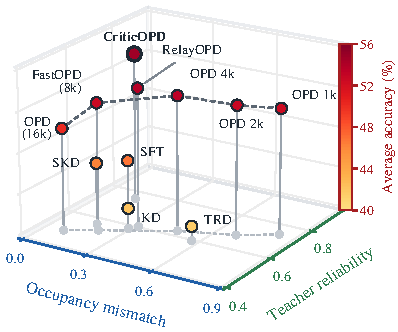
\includegraphics[width=\columnwidth]{figures/fig_mismatch.pdf}
\caption{Occupancy mismatch and teacher reliability on the states that each method supervises, and the average accuracy of the Qwen3-1.7B student.}
\label{fig:mismatch-reliability}
\end{figure}

\noindent\textbf{Reliability and occupancy mismatch together determine accuracy.}
Figure~\ref{fig:mismatch-reliability} places each method by the occupancy mismatch and the teacher reliability on the states that it supervises, and it marks the average accuracy of the Qwen3-1.7B student.
The occupancy mismatch is the total variation distance between the token positions of the prefixes that a method supervises and those of the prefixes that the student reaches at inference.
This distance is a lower bound on the true mismatch, and it shows which part of the response the supervision covers.
The teacher reliability is the mean recoverability of the teacher on the supervised states (Appendix~\ref{app:occupancy}).
\ours{} has an occupancy mismatch of $0.16$, which is slightly above $0.10$ for OPD but below $0.21$ for FastOPD and $0.35$ for RelayOPD.
FastOPD does not supervise positions after $8{,}192$ tokens, and RelayOPD ends the rollout after the second takeover, so both remove the later part of the response that the student reaches at inference.
The rewrite of \ours{} instead runs from the cut point to the end of the response.
A shorter length limit for OPD also increases the occupancy mismatch, and the accuracy stops improving beyond 8k tokens.
% TODO: verify the previous sentence against Figure~\ref{fig:mismatch-reliability}.
\ours{} combines the highest teacher reliability with a low occupancy mismatch and reaches the highest average accuracy.

\noindent\textbf{The critique gives credit to the correction.}
For each token of the rewrite, the advantage in Equation~\eqref{eq:fb} decomposes exactly as
\begin{equation}
\begin{aligned}
A_t^{\mathrm{fb}}
={}&
\underbrace{\log\pi_T(\tilde{y}_t\mid\tilde{h}_t)-\log\pi_\theta(\tilde{y}_t\mid\tilde{h}_t)}_{\text{OPD advantage}}\\
&+
\underbrace{\log\frac{\pi_T(\tilde{y}_t\mid\tilde{h}_t,c)}{\pi_T(\tilde{y}_t\mid\tilde{h}_t)}}_{r_t}.
\end{aligned}
\label{eq:fb-decomp}
\end{equation}
The first term is the advantage of OPD on the same sequence, and the second term $r_t$ is the pointwise mutual information between the token and the critique under the teacher.
Feedback distillation is therefore OPD on the rewrite with an additional reward $r_t$ on each token, and through this reward the teacher turns its recognition of errors into token-level credit.
To measure this credit, we compare two continuations of $64$ tokens at $132$ cut points, of which one continues the error and the other corrects it.
Under the scoring of OPD, the correction leads by only $0.24$ per token (95\% CI $[0.19, 0.29]$), whereas under the scoring of \ours{}, it leads by $1.47$ ($[1.36, 1.58]$; Figure~\ref{fig:why}(a)).
The first $32$ tokens account for $87\%$ of this increase.
A teacher without the critique thus barely separates the correction from the error, which is consistent with the drop of 1.19 points when the teacher scores the suffix without the feedback (Section~\ref{sec:experiments-ablation}).
The credit from the critique does not depend on which model writes the suffix, so a suffix that the teacher writes receives similar credit, consistent with the smaller drop of 0.66 points in that case.

\begin{figure}[t]
\centering
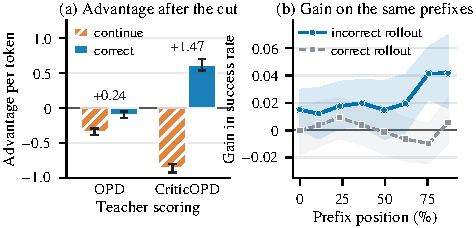
\includegraphics[width=\columnwidth]{figures/fig_mechanism.pdf}
\caption{(a) Advantage per token of two continuations of $64$ tokens at the cut point, which either continue or correct the error, under the scoring of OPD and of \ours{}. Numbers give correct minus continue. (b) Success rate of the student of \ours{} minus that of OPD from the same prefixes on OlympiadBench, with 95\% confidence bands.}
\label{fig:why}
\end{figure}

\noindent\textbf{The student learns to recover from its own errors.}
We take $150$ incorrect and $150$ correct rollouts of the initial student on OlympiadBench, which is not part of the training data, and let the students of OPD and \ours{} continue $16$ times from the empty prefix and each cut point.
The two students differ by at most $0.015$ on the empty prefix and by $0.000$ on average on correct prefixes.
On incorrect prefixes, the student of \ours{} leads by $0.023$ on average ($[0.010, 0.036]$) and by about $0.04$ at the last two cut points (Figure~\ref{fig:why}(b)).
The gain therefore concentrates on the states after the student errs, which are the states where the supervision of OPD loses its reliability in Section~\ref{sec:diagnosis}.
This behavior also lengthens the responses, so part of the gain comes with longer reasoning, but at the same response length the critique still improves the student (Appendix~\ref{app:budget}).